\documentclass{report}
\usepackage[english]{babel}
%Package for images
\usepackage{graphicx}
%graphicx folder
\graphicspath{images/}
%Package for math
\usepackage{amsmath,amssymb,amsfonts,textcomp,amsthm,mathrsfs}
\usepackage{url}

%Used for defining own colours for the chapter numbering and sections colours
\usepackage{xcolor}
%For quotes at the beginning of chapters
\usepackage{epigraph}
%External linking
\usepackage{hyperref}
%Pakket voor itemize deftig te maken
\usepackage{enumitem}
%Random text generator
\usepackage{lipsum}
%To be able to wrap text around figures
\usepackage{wrapfig}

% Page layout
\usepackage[a4paper,width=150mm,top=25mm,bottom=25mm]{geometry}

%Package for codes
\usepackage{minted}

%Use subfigures
\usepackage{caption}
\usepackage{subcaption}

% Chapter and section formatting
\usepackage{titlesec}
\titleformat{\chapter}[display]{\normalfont\bfseries\color[RGB]{0, 71, 171}\Huge}{\chaptertitlename\ \thechapter}{20pt}{\Huge}

\titleformat{\section}[block]{\normalfont\bfseries\color[RGB]{0, 71, 171}\Large}{\thesection}{10pt}{\Large}

\titleformat{\subsection}[block]{\normalfont\bfseries\color[RGB]{0,71,171}\large}{\thesubsection}{10pt}{\large}

\titlespacing*{\chapter}{0pt}{0pt}{20pt}

% Title page
\begin{document}
%begin titlepage
\begin{titlepage}
    \begin{center}
        
\includegraphics[width=0.5\textwidth]{images/logo_UGent_EN_RGB_2400_color.png}
        
        \huge 
        \text{Faculty Of Sciences}
        
        \Huge
        \textbf{Dynamical analysis of a dark-matter halo and galaxies in cosmological, hydrodynamical simulations.}
        
        \vspace{0.2cm}
        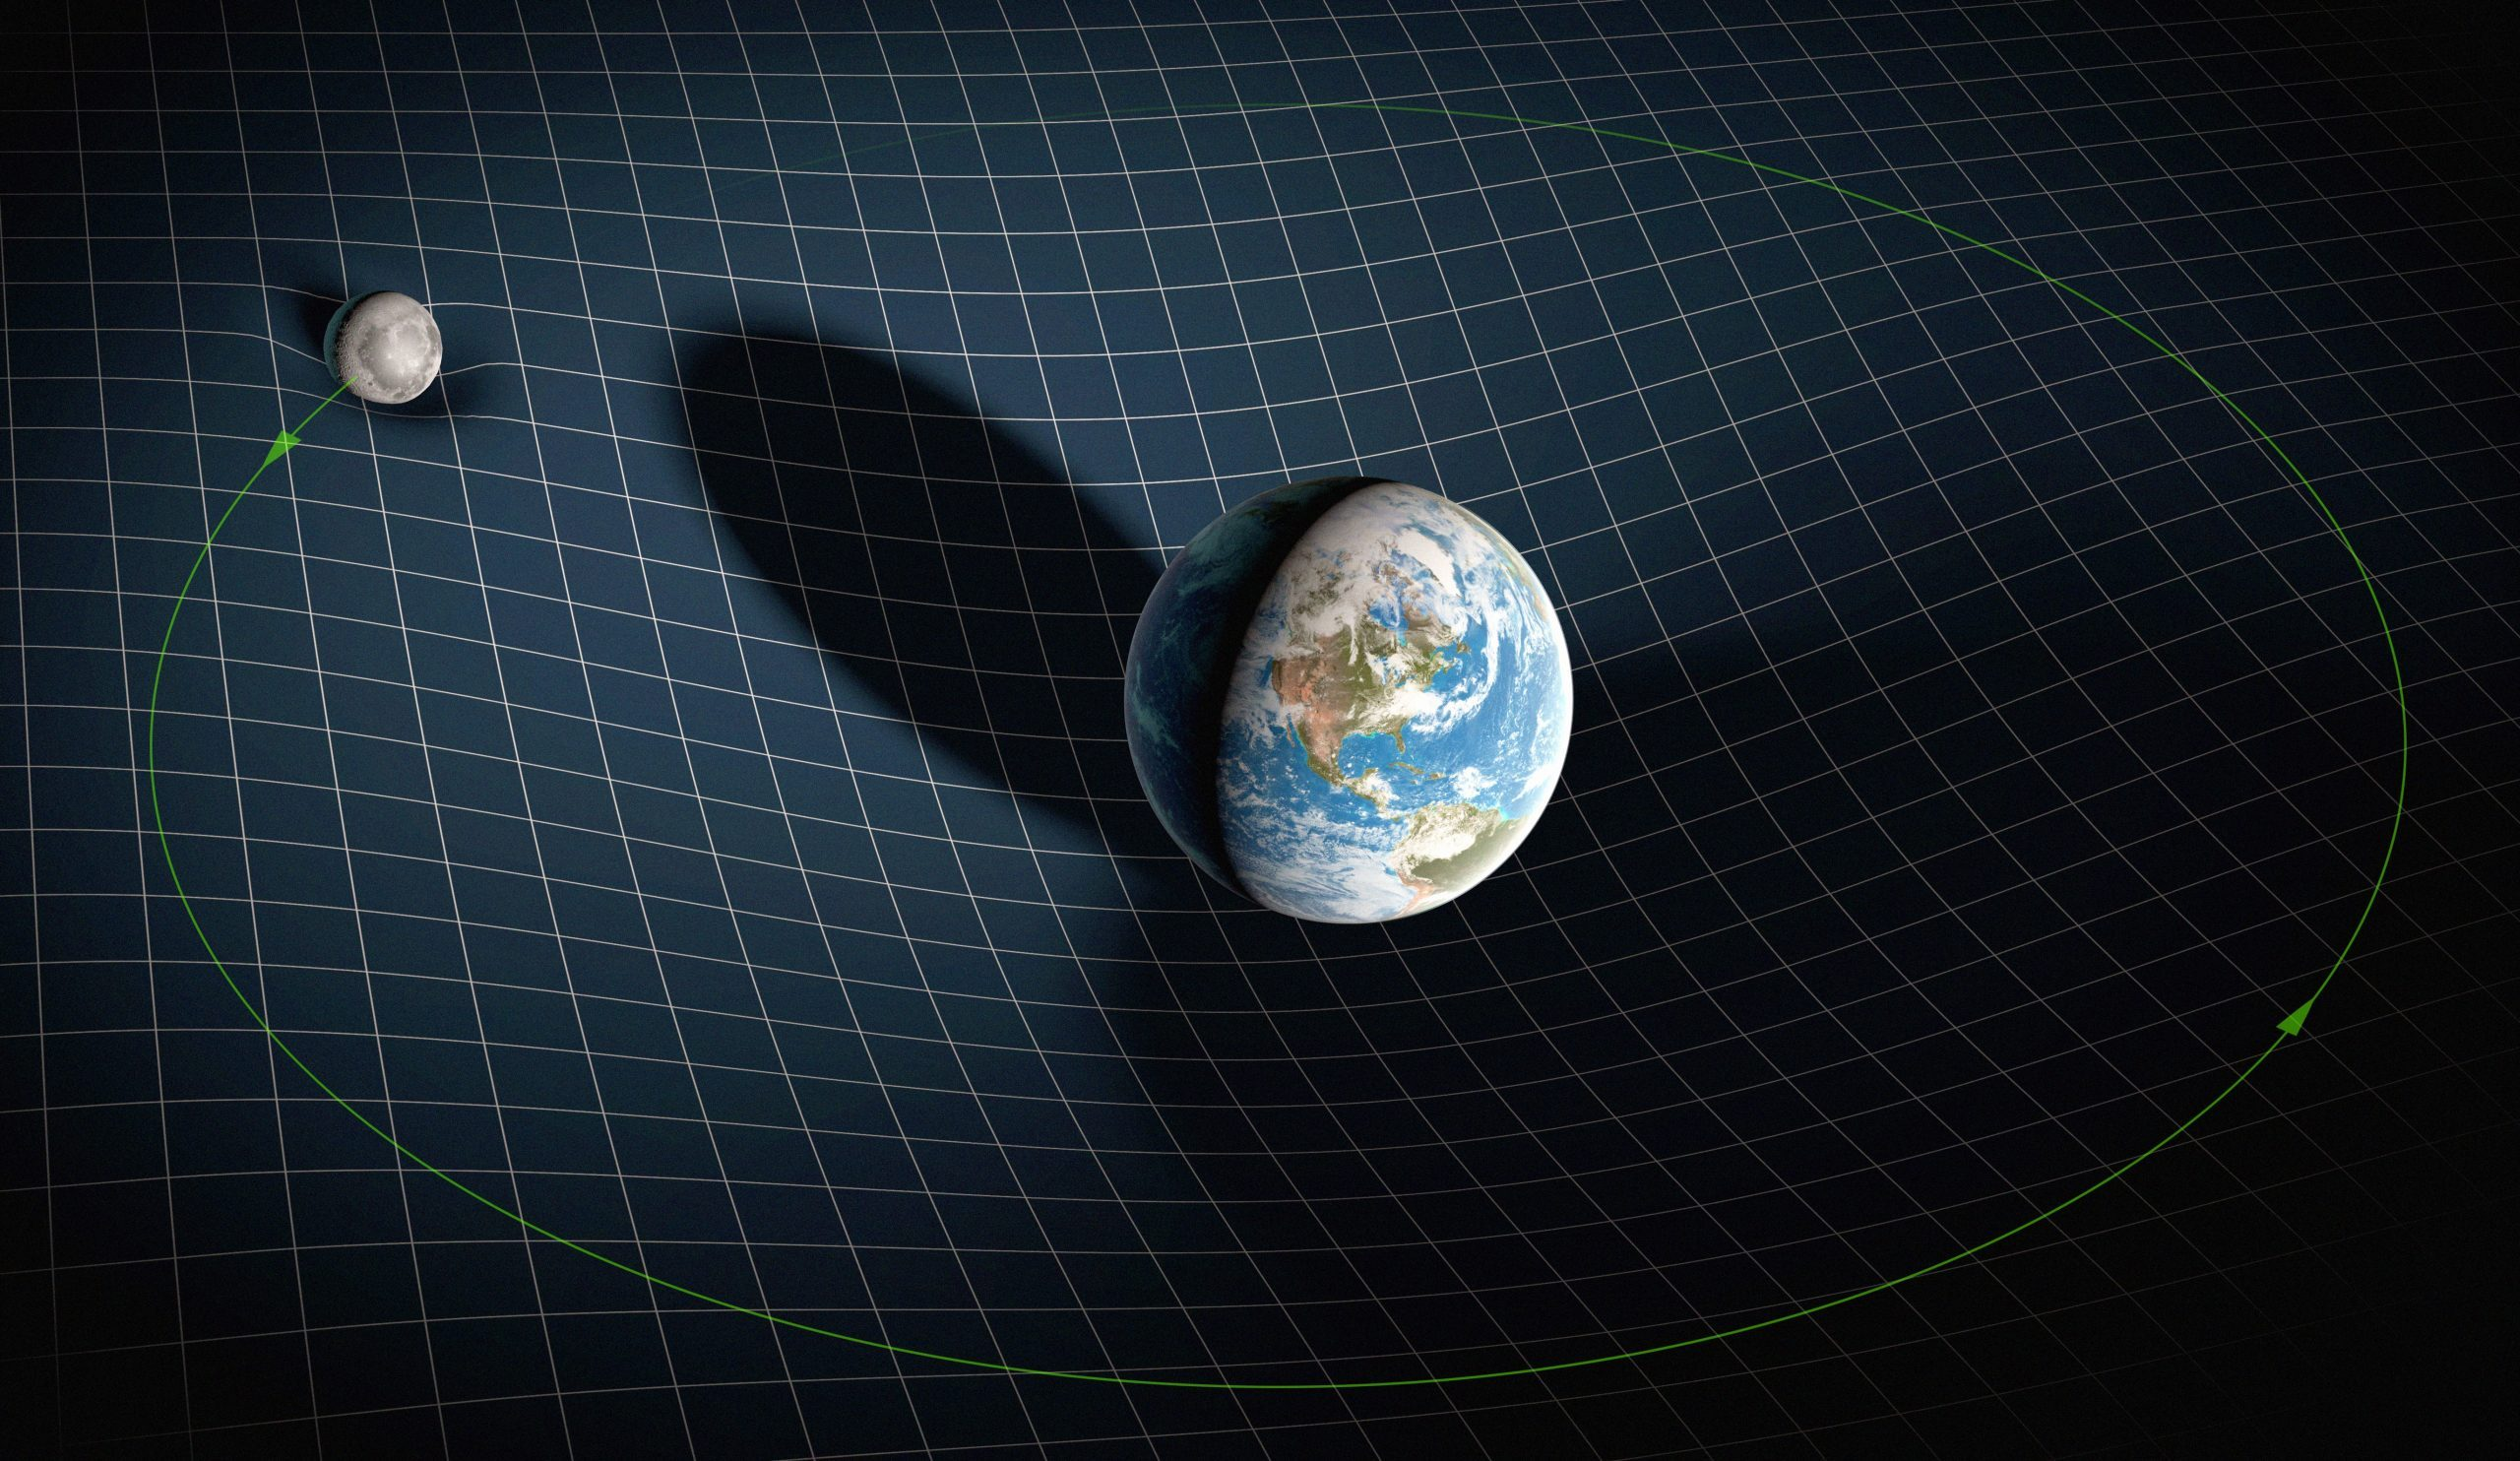
\includegraphics[width=12cm, height = 8cm]{images/Gravity-9b985a4-scaled.jpg}
        
        \vspace{0.2cm}
        \Large
        \textbf{Boateng Christopher, Verheecke Jitske}
        
        \vspace{0.5cm}
        \normalsize
        Master of Science in Physics and Astronomy\\
        
        \vspace{0.5cm}
        \large Department of Physics and Astronomy - WE05
        
        \vspace{0.1cm}
        \large October 2025
    \end{center}
\end{titlepage}
%end titlepage


% Table of contents
\pagenumbering{roman}
\tableofcontents

% Chapters
\thispagestyle{plain}
\begin{center}
    \Large
    \textbf{Dynamical analysis of a dark-matter halo and galaxies in cosmological, hydrodynamical simulations.}

    \vspace{0.4cm}
    \textbf{Boateng Christopher, Verheecke Jitske}
    
    \vspace{0.9cm}
    \textbf{Abstract}
\end{center}

\vspace{0.5cm}
\noindent\textbf{Keywords:}

\clearpage
\pagenumbering{arabic}
\setcounter{page}{1}
\chapter{Introduction}
\section{Cosmology}
\subsection{Cosmological parameters}
\begin{equation}
1 + z = \frac{1}{a}
\end{equation}
\begin{equation}
\Omega_m (z) = \frac{\Omega_{m,0} (1+z)^3}{\Omega_{m,0} (1+z)^3 + \Omega_{\Lambda,0}}
\end{equation}

\subsection{Unit system}
\begin{equation}
    kpc, M_\odot, Gyr
\end{equation}


\chapter{Methodology}
\chapter{Results and Discussion}
%\chapter{Discussion}
\chapter{Conclusion}
\appendix
\chapter{Appendix}
\subsection{Scripts}

\bibliographystyle{ieeetr}
\bibliography{ref}

\end{document}
